% !TEX encoding = UTF-8 Unicode
\documentclass{beamer}

\usepackage{cmap}
\usepackage[parfill]{parskip}
\usepackage{polyglossia}
\usepackage[ruled,vlined]{algorithm2e}

% Related to math
\usepackage{amsmath,amssymb}
\usepackage{graphicx}
\usepackage{subcaption}

\setdefaultlanguage[spelling=modern]{russian}
\setotherlanguage{english}
\setmainfont{FreeSans}
\setsansfont{FreeSerif}
\setmonofont{FreeMono}

\addtobeamertemplate{navigation symbols}{}{%
    \usebeamerfont{footline}%
    \usebeamercolor[fg]{footline}%
    \hspace{1em}%
    \insertframenumber/\inserttotalframenumber
}


\title{Greedy Sparse Least-Squares SVM}
\author{Сон Артём}

\begin{document}
\maketitle

\begin{frame}
	\frametitle{Постановка задачи}
	\begin{itemize}
		\item Пусть дано множество тренировочных данных:
		      $ \mathcal{D} = {(x_i, y_i)}_{i = 1}^{l}, x_i \in \mathcal{X} \subset
			      \mathbb{R}^d, y_i \in \mathcal{Y} \subset \mathbb{R}$
		\item Необходимо найти функцию $f(x)$, которая наилучшим образом
		      предсказывает новые наблюдения.
		\item Модель нелинейной регрессии с квадратичной функцией
		      потерь задается следующим образом:
		      \begin{itemize}
			      \item $\mathcal{K}(x, x^{\prime}) = \phi(x) \cdot \phi(x^\prime), \;$
			            - ядерная функция
			            \begin{itemize}
				            \item $\mathcal{K} : \mathcal{X} \times \mathcal{X}
					                  \rightarrow \mathbb{R}$
				            \item $\phi: \mathcal{X} \rightarrow \mathcal{F}, \;
					                  \mathcal{F} \;$  - пространство признаков высшей
				                  размерности
			            \end{itemize}
			      \item $W_{LS-SVM}(w, b) = \frac{1}{2} ||w||^2 + \frac{\gamma}{l}
				            \sum_{i = 1}^{l}(y_i - w \cdot \phi(x_i) + b)^2$
			            - целевая функция модели,
			            $w = \sum_{i=1}^{l} \alpha_i \phi(x_i)$
			      \item $f(x) = \sum_{i = 1}^{l} \alpha_i \mathcal{K}(x_i, x) + b$ -
			            решающая функция, полученная минимизацией целевой функции.
		      \end{itemize}
	\end{itemize}

\end{frame}

\begin{frame}
	\frametitle{Идея алгоритма}

	\begin{itemize}
		\item Пусть даны тренировочные данные:
		      $ \mathcal{D} = {(x_i, y_i)}_{i = 1}^{l}, x_i \in \mathcal{X} \subset
			      \mathbb{R}^d, y_i \in \mathcal{Y} \subset \mathbb{R}$
		\item Дана модель нелинейной регресси с квадратичной функции потерь,
		      c ядерной функцией $\mathcal{K} : \mathcal{X} \times
			      \mathcal{X} \rightarrow \mathbb{R}$,
		      определяющую коэффициенты $\{b, \alpha_i\}_{i =
			      1}^{l} \subset \mathbb{R}$
		      решающей функции
		      $f(x) = \sum_{i = 1}^{l} \alpha_i \mathcal{K}(x_i,
			      x) + b$, минимизируя целевую функцию модели

	\end{itemize}

	Мы хотим найти такое приближение, что для некоторого
	подмножества $S \subset \{1, \; ... \; , l \}$, коэффициенты $\{b,
		\beta_i\}_{i=1}^{l} \subset \mathbb{R}$ будут минимизировать функцию
	цели $f(x) = \sum_{i \in S} \beta_i \mathcal{K}(x_i, x) + b$
	нашей GSLS-SVM модели с параметром регуляризации $\gamma$:
	\vspace{-10pt}
	\begin{equation*}
		\mathcal{L}(\beta, b) = \frac{1}{2} \sum_{i,j \in S} \beta_i \beta_j
		\mathcal{K}(x_i, x_j)
		+ \frac{\gamma}{l} \sum_{i=1}^{l} (y_i - \sum_{j \in S} \beta_j
		\mathcal{K}(x_i, x_j))^2
	\end{equation*}

\end{frame}

\begin{frame}
	\frametitle{Алгоритм. Жадность}
	\begin{itemize}
		\item Каждую итерацию GSLS выбирается новый вектор из датасета в качестве
		      опорного
		\item Вычисляется целевая функция, и лучший на данной итерации
		      опорный вектор добавляется к результирующему поднможеству.
		\item Процесс завершается, когда в подмножество достигло некоторого
		      предопределенного размера.
	\end{itemize}
\end{frame}

\begin{frame}
	\frametitle{Алгоритм. Вычисления (1)}
	\begin{equation*}
		\mathcal{L}(\beta, b) = \frac{1}{2} \sum_{i,j \in S} \beta_i \beta_j
		\mathcal{K}(x_i, x_j)
		+ \frac{\gamma}{l} \sum_{i=1}^{l} (y_i - \sum_{j \in S} \beta_j
		\mathcal{K}(x_i, x_j))^2
	\end{equation*}

	Если приравнять частные производные по $\beta$ и $b$ нулю, и разделить на
	$2\gamma / l$, получим:
	\begin{equation*}
		\sum_{i \in S}\beta_i \sum_{j = 1}^{l}k_{ij} + lb = \sum_{j=1}^{l}y_j
	\end{equation*}
	и
	\[
		\sum_{i \in S} \beta_i \{ \frac{l}{2\gamma} k_{ir} + \sum_{j = 1}^{l}k_{jr}
		k_{ji}\} + b \sum_{i=1}^{l}k_{ir} = \sum_{i=1}^{l}y_i k_{ir} \quad
		\forall r \in S
	\]

\end{frame}

\begin{frame}
	\frametitle{Алгоритм. Вычисления (2)}

	Эти уравнения представляют из себя СЛАУ с $|S| + 1$ уравнениями и
	неизвестными. В матричной форме:
	\begin{equation*}
		H \begin{bmatrix}
			\beta \\
			b
		\end{bmatrix} =
		\begin{bmatrix}
			\Omega & \Phi \\
			\Phi^T & l
		\end{bmatrix}
		\begin{bmatrix}
			\beta \\
			b
		\end{bmatrix}
		= \begin{bmatrix}
			c \\
			\sum_{k = 1}^{l} y_k
		\end{bmatrix},
	\end{equation*}

	\vspace{-20pt}
	\begin{flushleft}
		\begin{align*}
			\text{где} \quad & \Omega = [ \frac{l}{2\gamma}k_{ij} + \sum_{r = 1}^{l} k_{rj} k_{ri}
			]_{i,j \in S},                                                                         \\
			                 & \Phi = (\sum_{j=1}^{l}k_{ij})_{i \in S},                            \\
			                 & c = ( \sum_{j=1}^{l}y_j k_{ij} )_{i \in S},                         \\
			                 & k_{ij} = \mathcal{K}(x_i, x_j)
		\end{align*}
	\end{flushleft}



\end{frame}

\begin{frame}
	\frametitle{Псеводкод}
	\begin{algorithm}[H]
		% \SetAlgoLined
		\KwData{$\mathcal{K},\; \mathcal{X},\; \mathcal{Y},\; sv\_num$}
		\KwResult{$S,\; \beta_{best},\; b_{best}$}

		$l = |\mathcal{X}|, \; \mathcal{L}_{best} = \infty$\;
		$S, \; \beta_{best},\; b_{best},\; index_{best} = \{\}$\;

		\While{$|S| \neq  sv\_num$}{
			\For{$j \in \mathcal{X} \backslash S$} {
				$S \leftarrow j$\;
				compute $\Omega, \; \Phi, \; c, \; H$\;
				$(\beta, \; b) = H^{-1} * (\sum_{k = 1}^l y_k, \; c) $\;
				L = $\mathcal{L}(\beta, b)$\;
				\If{L $< \mathcal{L}_{best}$} {
					$\beta_{best}, \; b_{best},\; \mathcal{L}_{best},\; index_{best} = \beta,
						\; b, \; L, \; j$ \;
				}

				$S \rightarrow j$ \;
			}
			$S \leftarrow index_{best}$\;
		}
	\end{algorithm}

\end{frame}
\begin{frame}
	\frametitle{Результаты}
	\begin{itemize}
		\item Во всех эксперементах использовалось Гауссовское ядро
		      $\mathcal{K}(x, x^\prime) = exp(- \frac{|x - x^\prime|}{2 \sigma^2})$
		\item Восстанавливалсь функция $sinc(x),\; l = 200$
		\item Регрессия восстанавливалась для количества опорных векторов $n = 3,\;
			      6,\; 7$ по точным данным, и данным с шумом
		\item Шум добавлялся нормальным распределенимем $N(0, 0.1)$
		\item Зависимость СКО от количества опорных векторов проводилась для $n = 1,
			      ..., 12$
		      \begin{itemize}
			      \item $\sigma = 0.7, \; \gamma = 10^5$
		      \end{itemize}


	\end{itemize}
\end{frame}

\begin{frame}
	\frametitle{Результаты. Графики (1)}
	\begin{figure}
		\centering
		\begin{subfigure}{0.4\textwidth}
			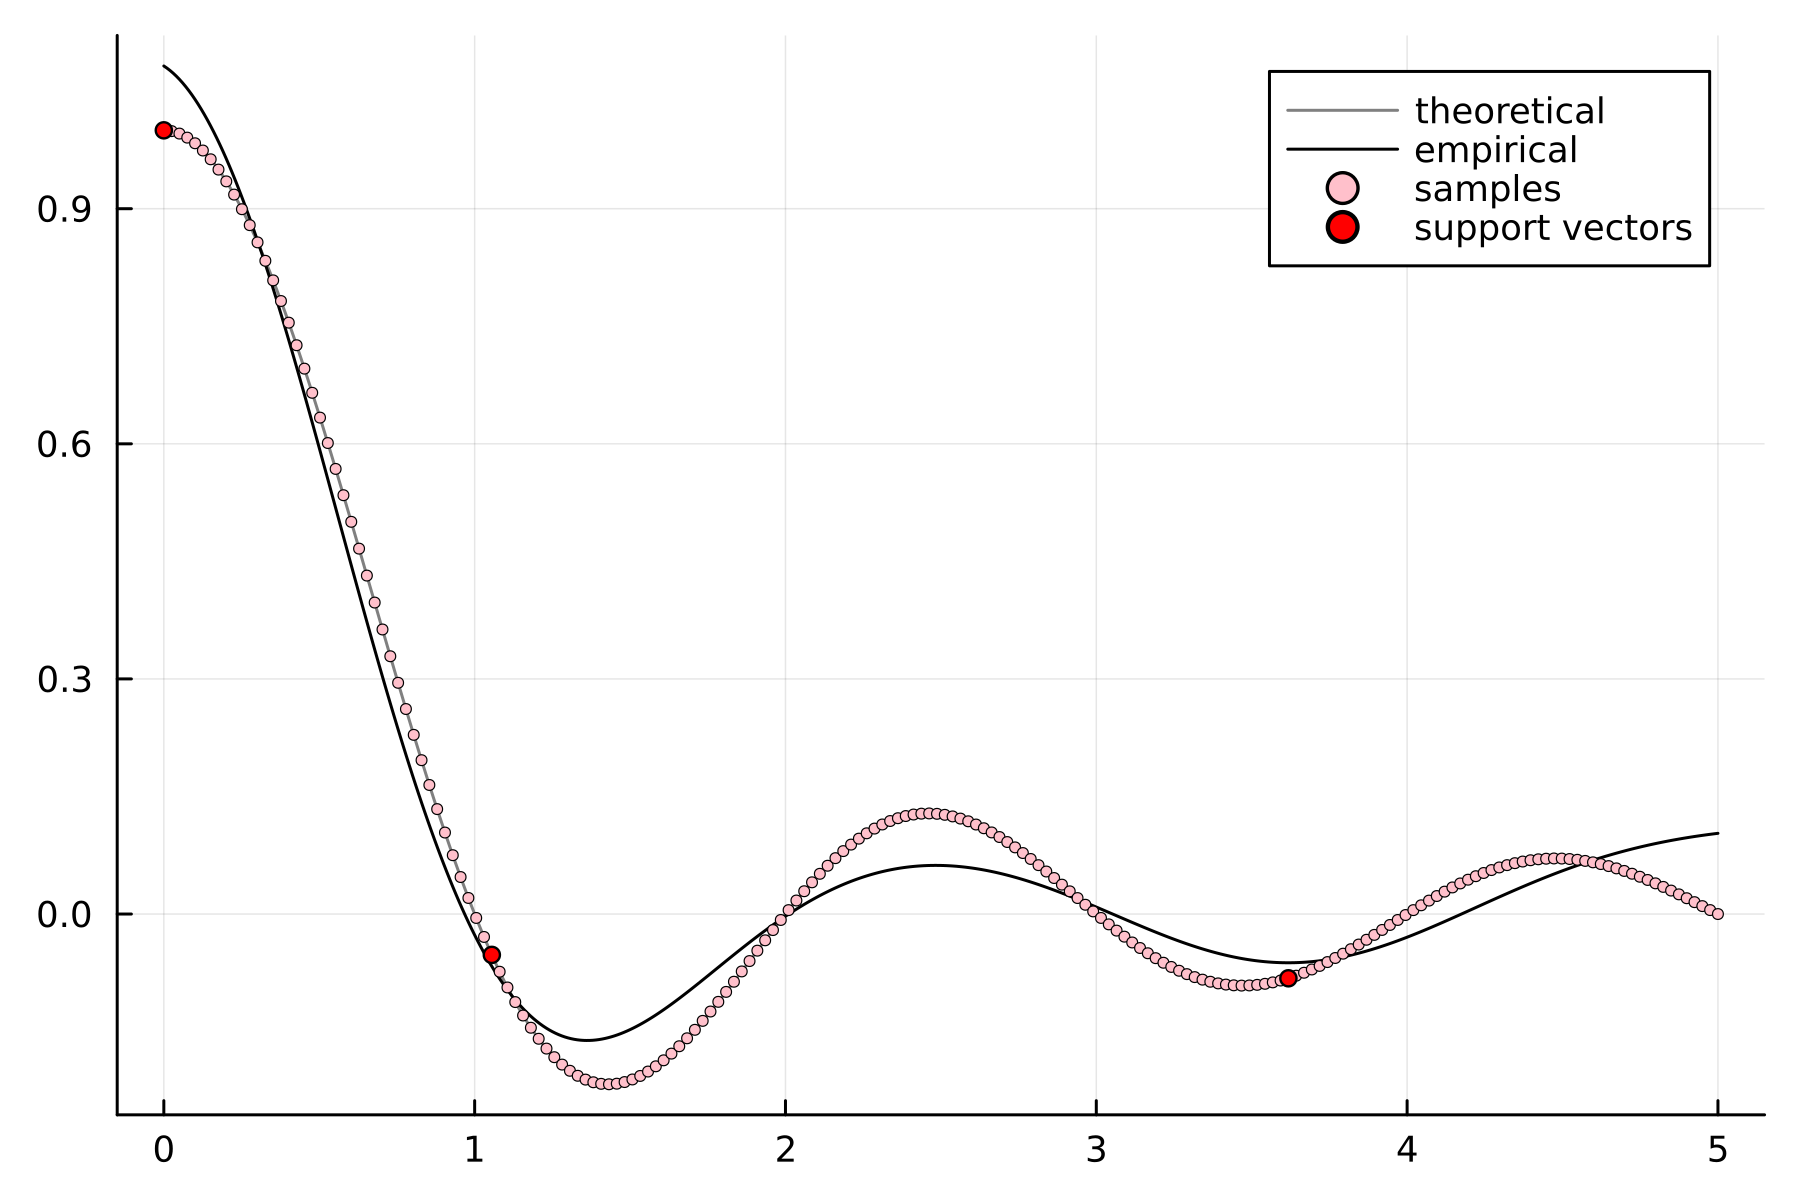
\includegraphics[width=\linewidth]{../model3.png}
			\caption{3 опорных вектора}
		\end{subfigure}
		\begin{subfigure}{0.4\textwidth}
			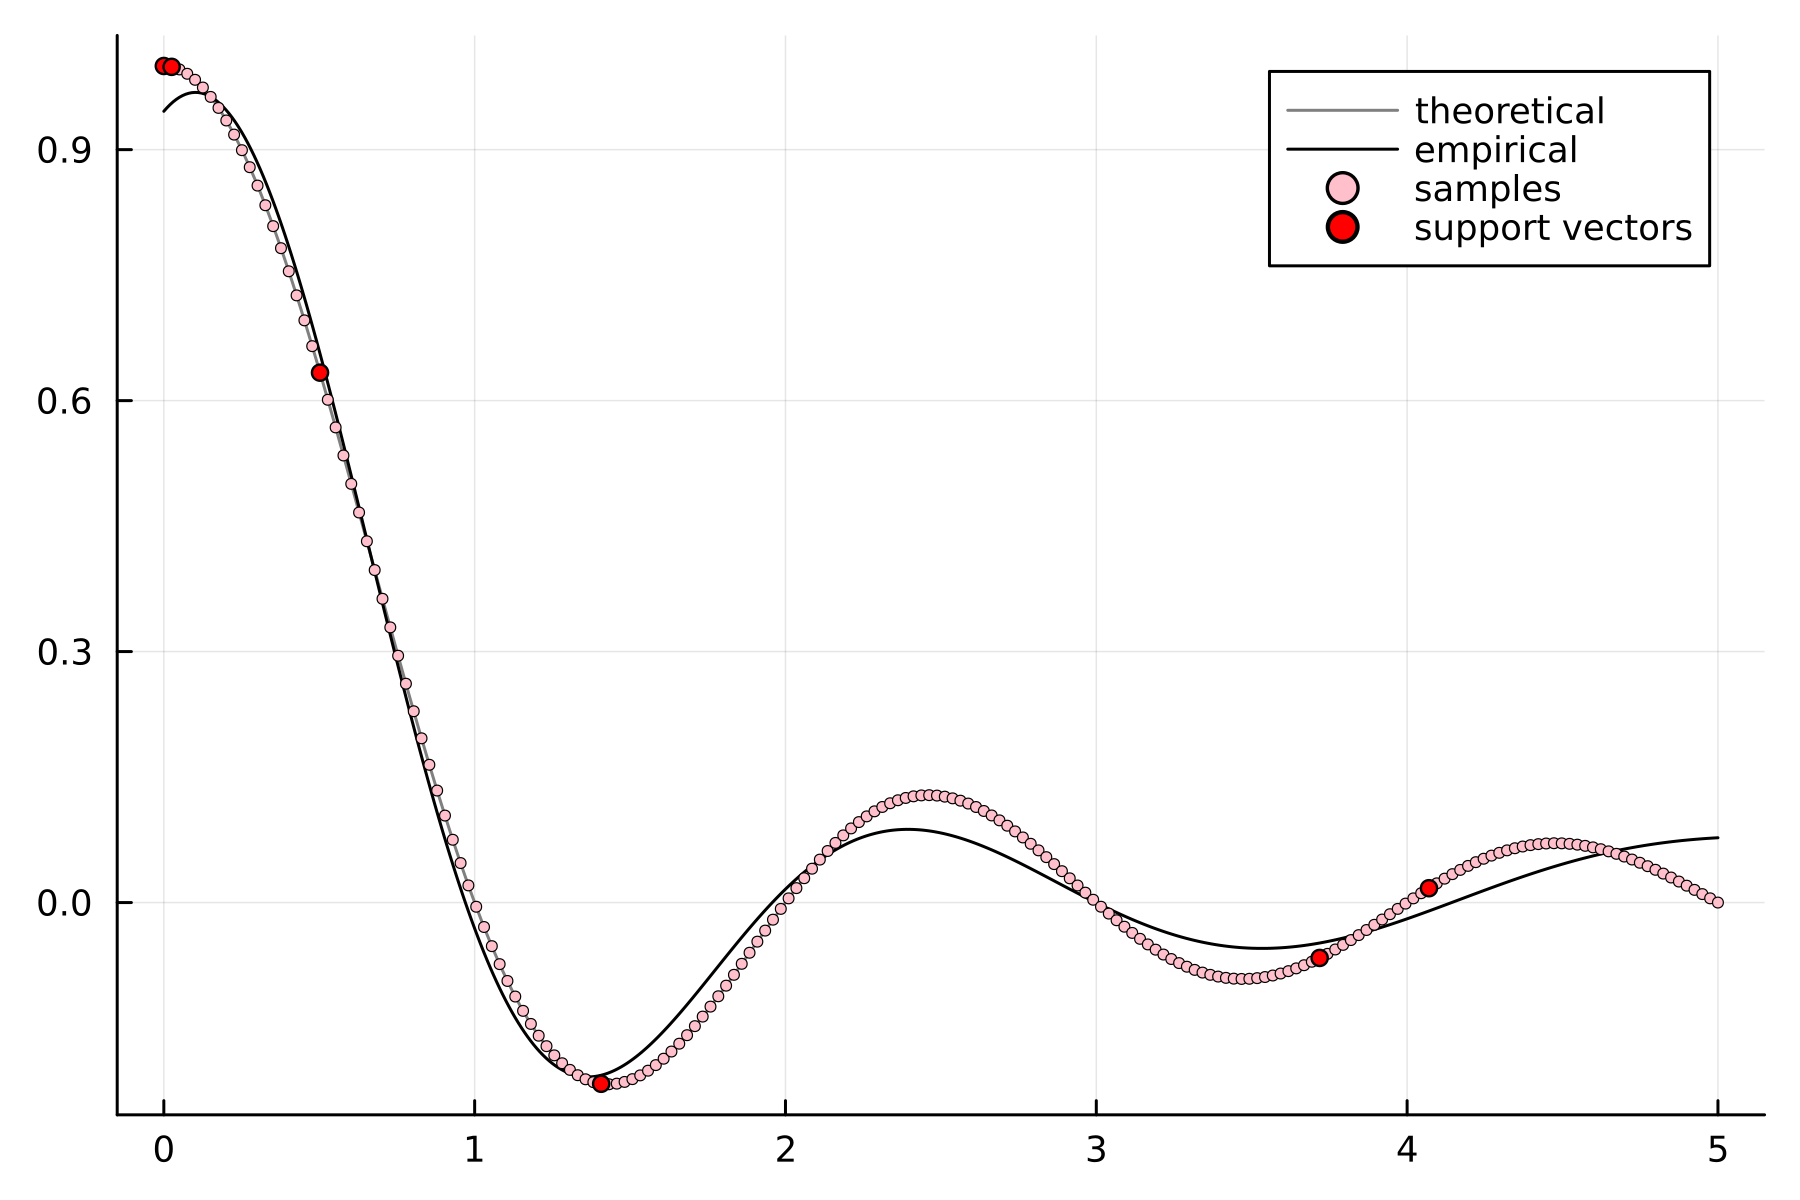
\includegraphics[width=\linewidth]{../model6.png}
			\caption{6 опорных вектора}
		\end{subfigure} \\
		\begin{subfigure}{0.4\textwidth}
			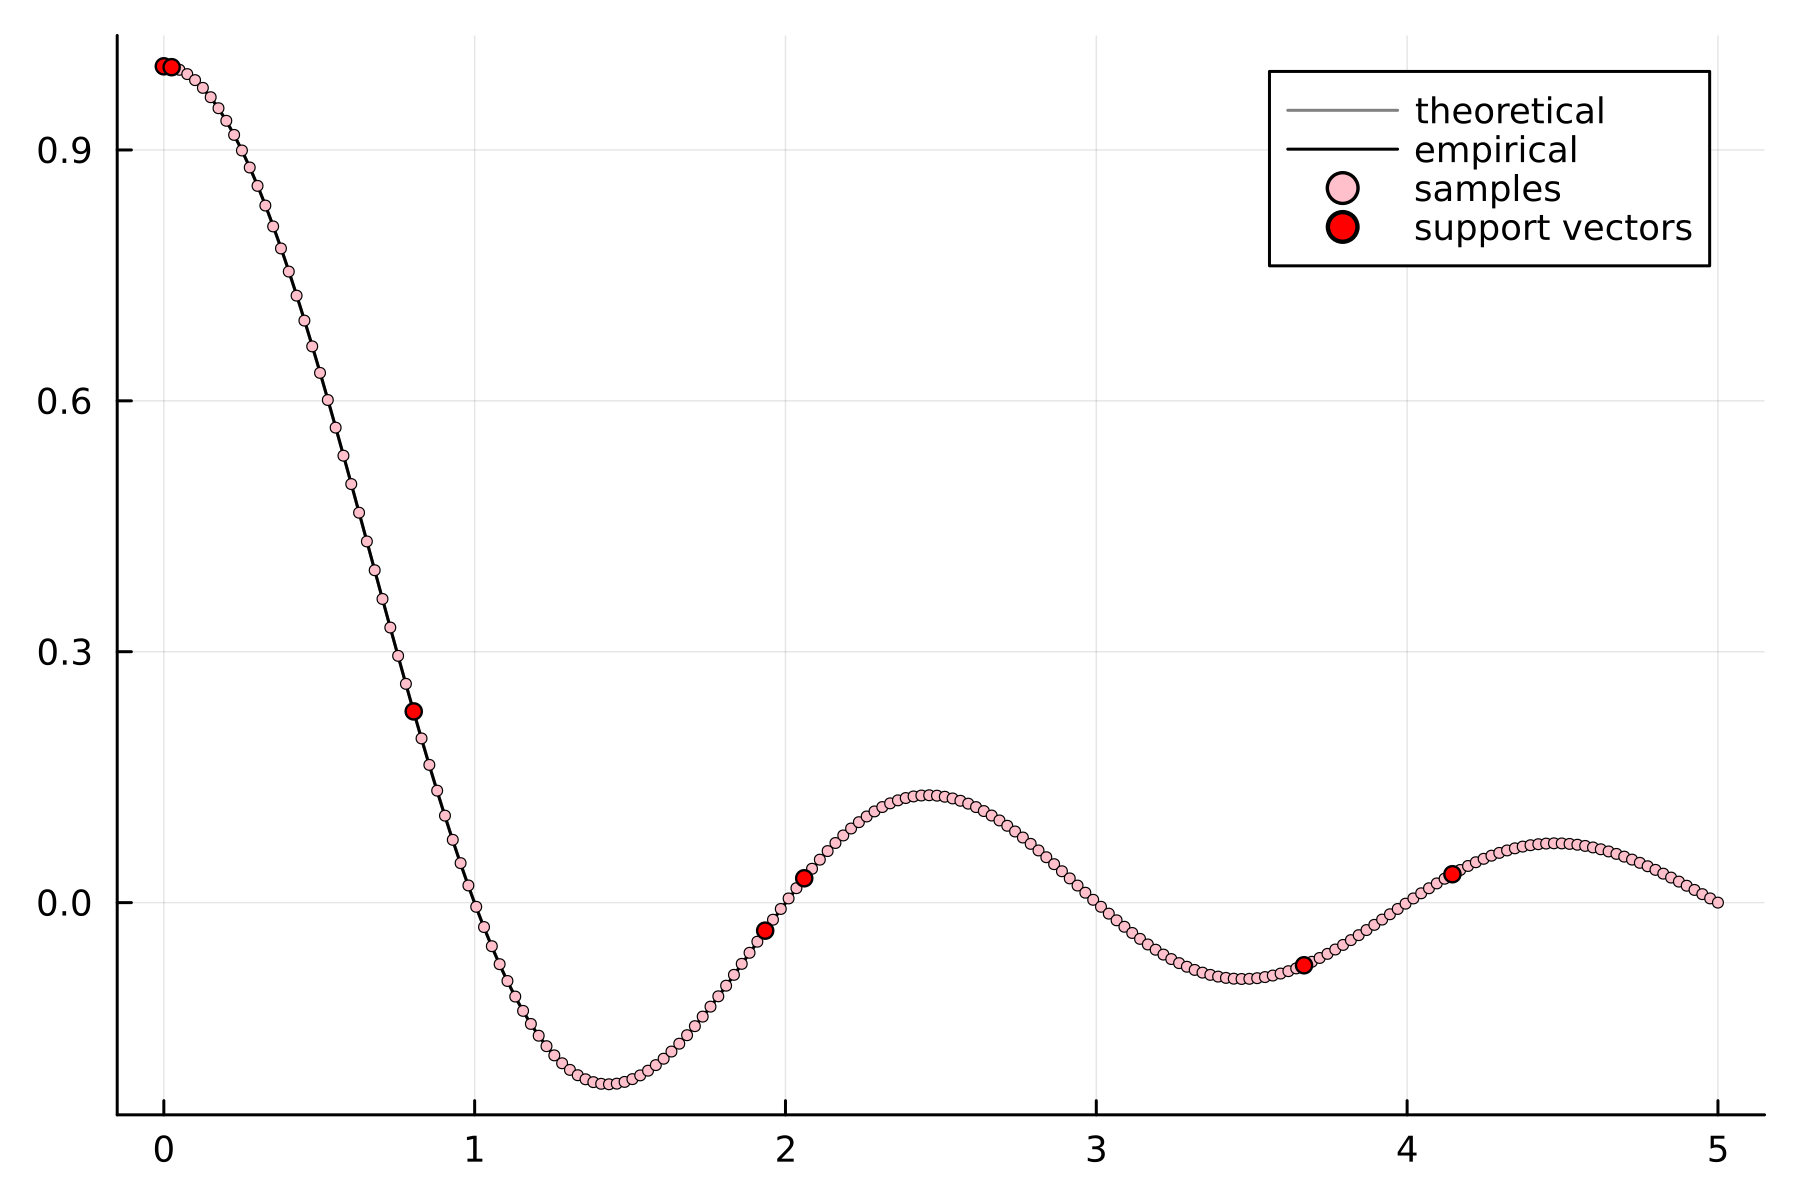
\includegraphics[width=\linewidth]{../model7.png}
			\caption{7 опорных вектора}
		\end{subfigure}
		\caption{Регрессия без шума}
	\end{figure}
\end{frame}

\begin{frame}
	\frametitle{Результаты. Графики (2)}
	\begin{figure}
		\centering
		\begin{subfigure}{0.4\textwidth}
			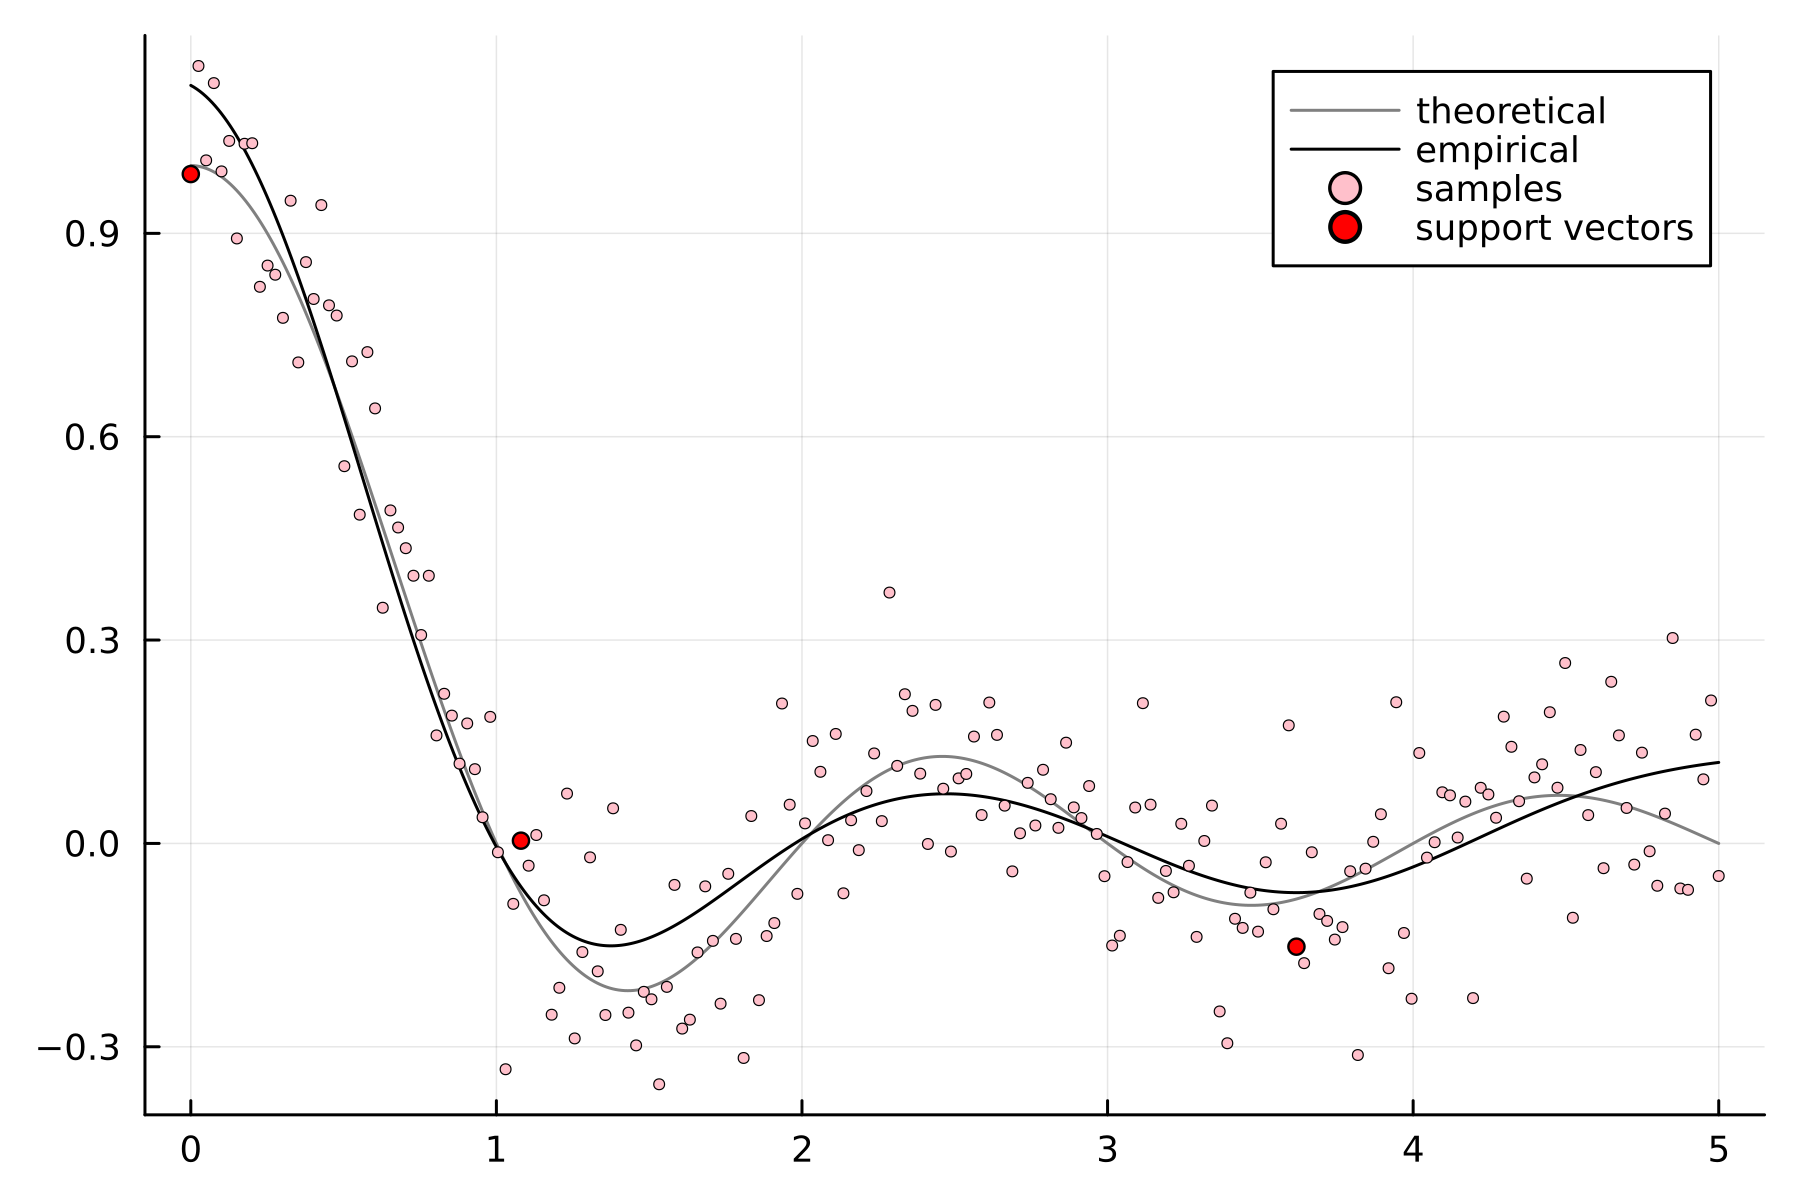
\includegraphics[width=\linewidth]{../model_noise3.png}
			\caption{3 опорных вектора}
		\end{subfigure}
		\begin{subfigure}{0.4\textwidth}
			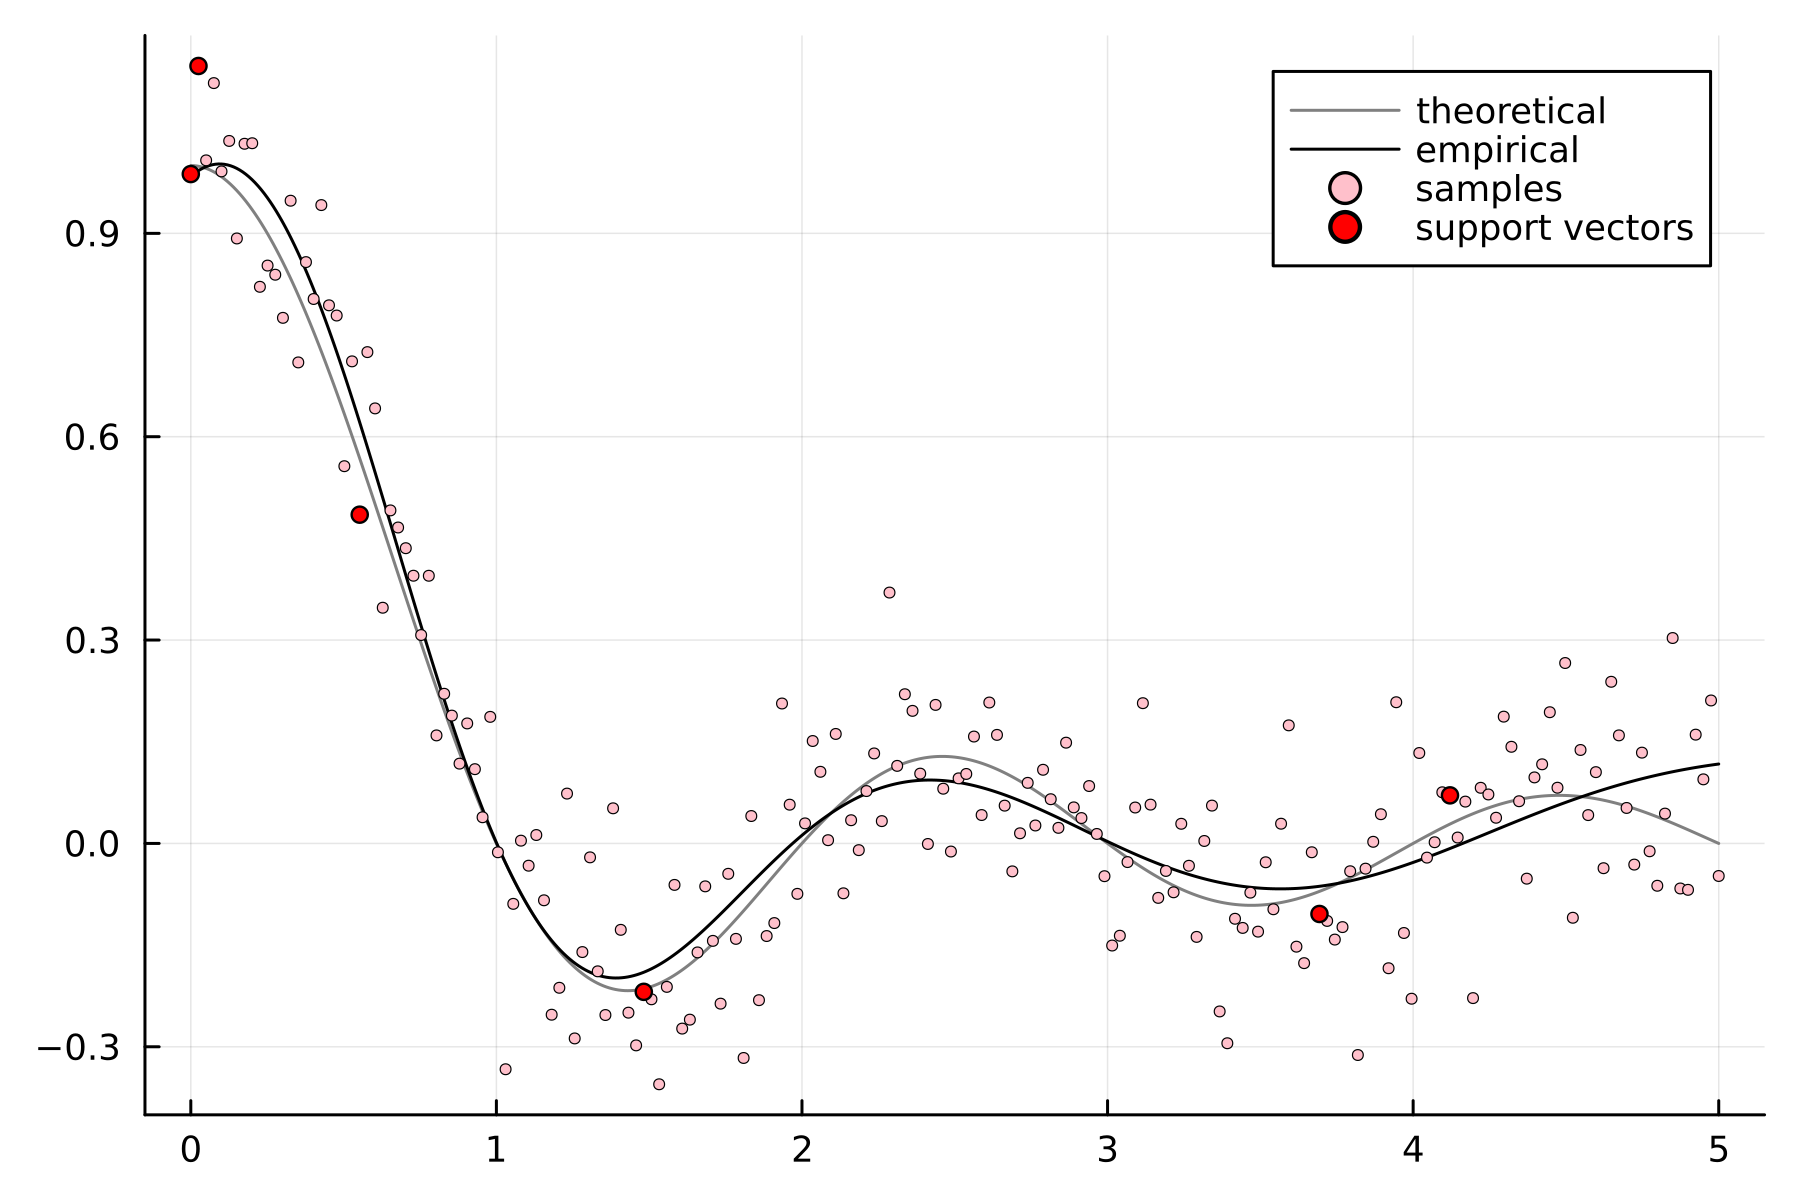
\includegraphics[width=\linewidth]{../model_noise6.png}
			\caption{6 опорных вектора}
		\end{subfigure} \\
		\begin{subfigure}{0.4\textwidth}
			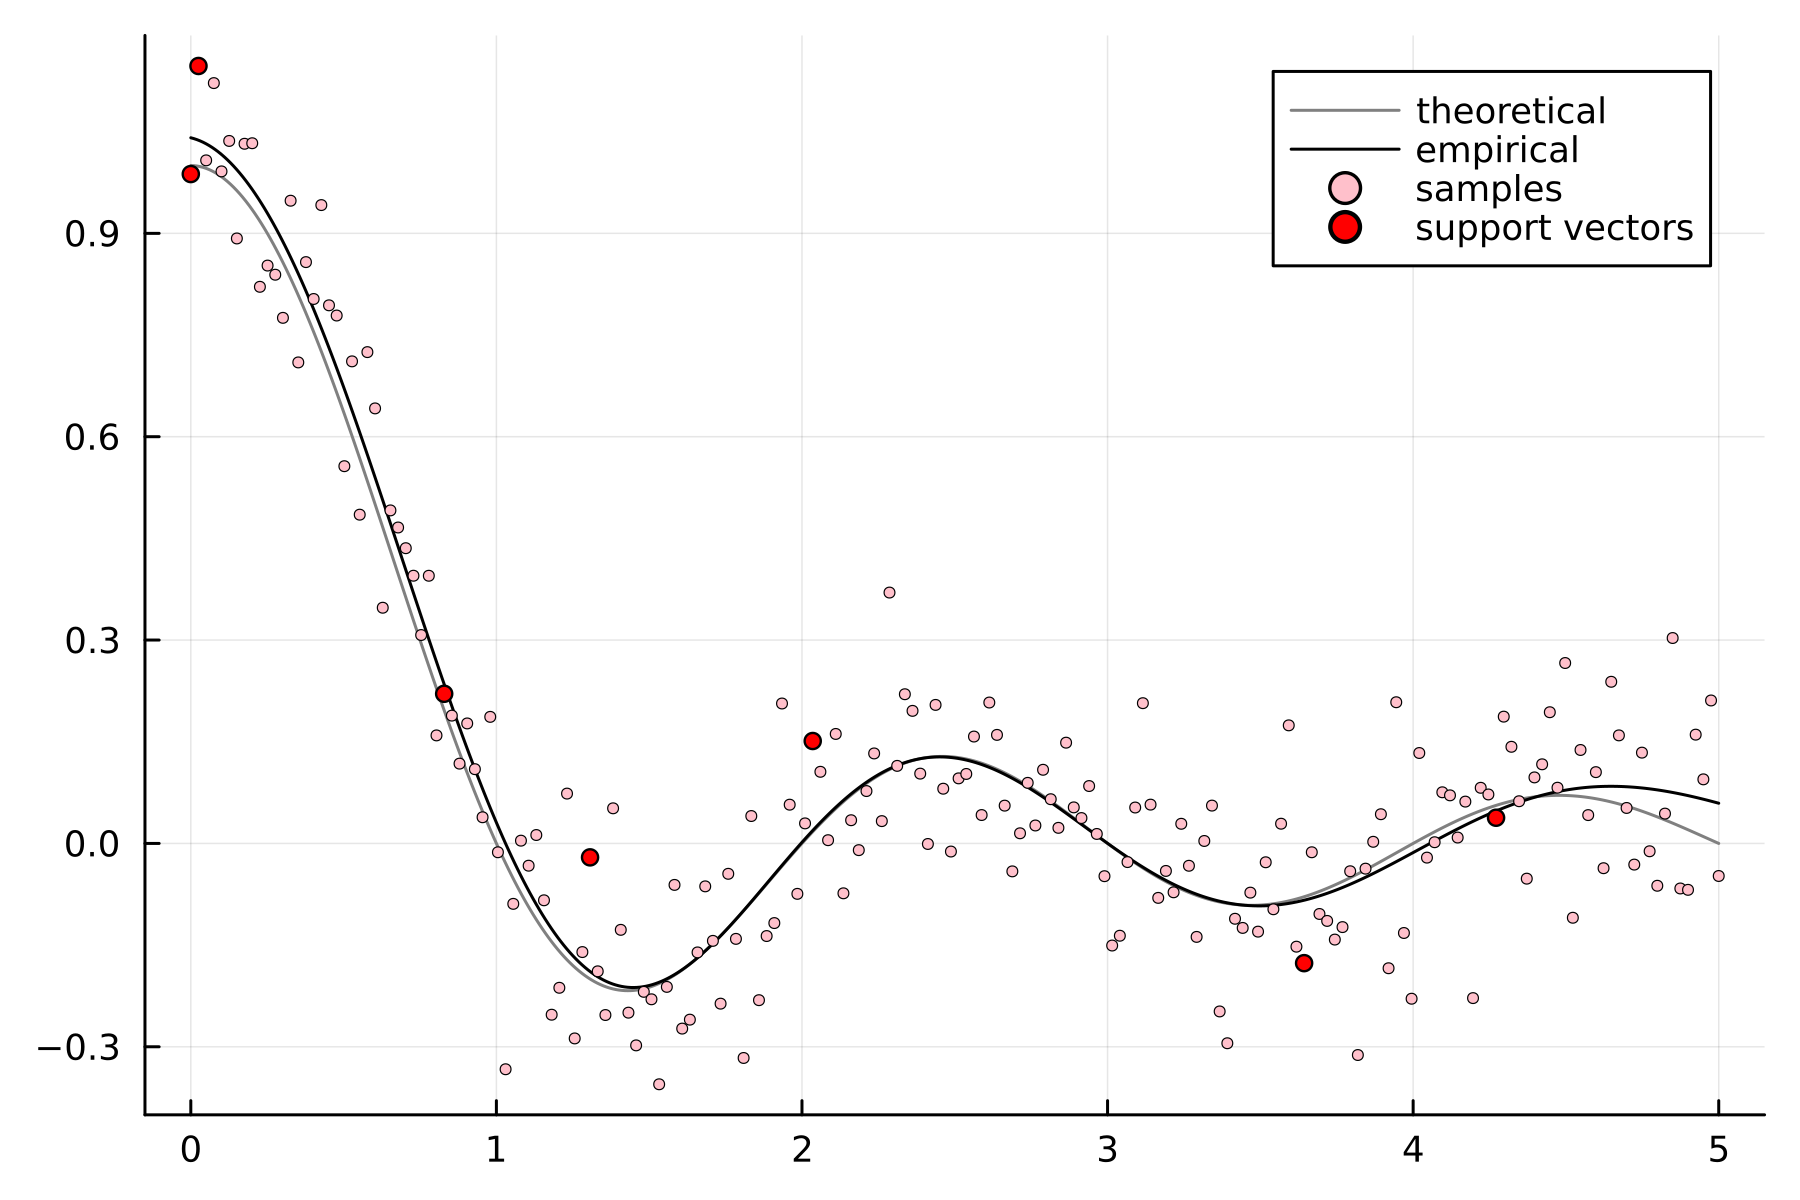
\includegraphics[width=\linewidth]{../model_noise7.png}
			\caption{7 опорных вектора}
		\end{subfigure}
		\caption{Регрессия c шумом}
	\end{figure}

\end{frame}

\begin{frame}
	\frametitle{Результаты. Графики (3)}
	\begin{figure}
		\centering
		\begin{subfigure}{0.4\textwidth}
			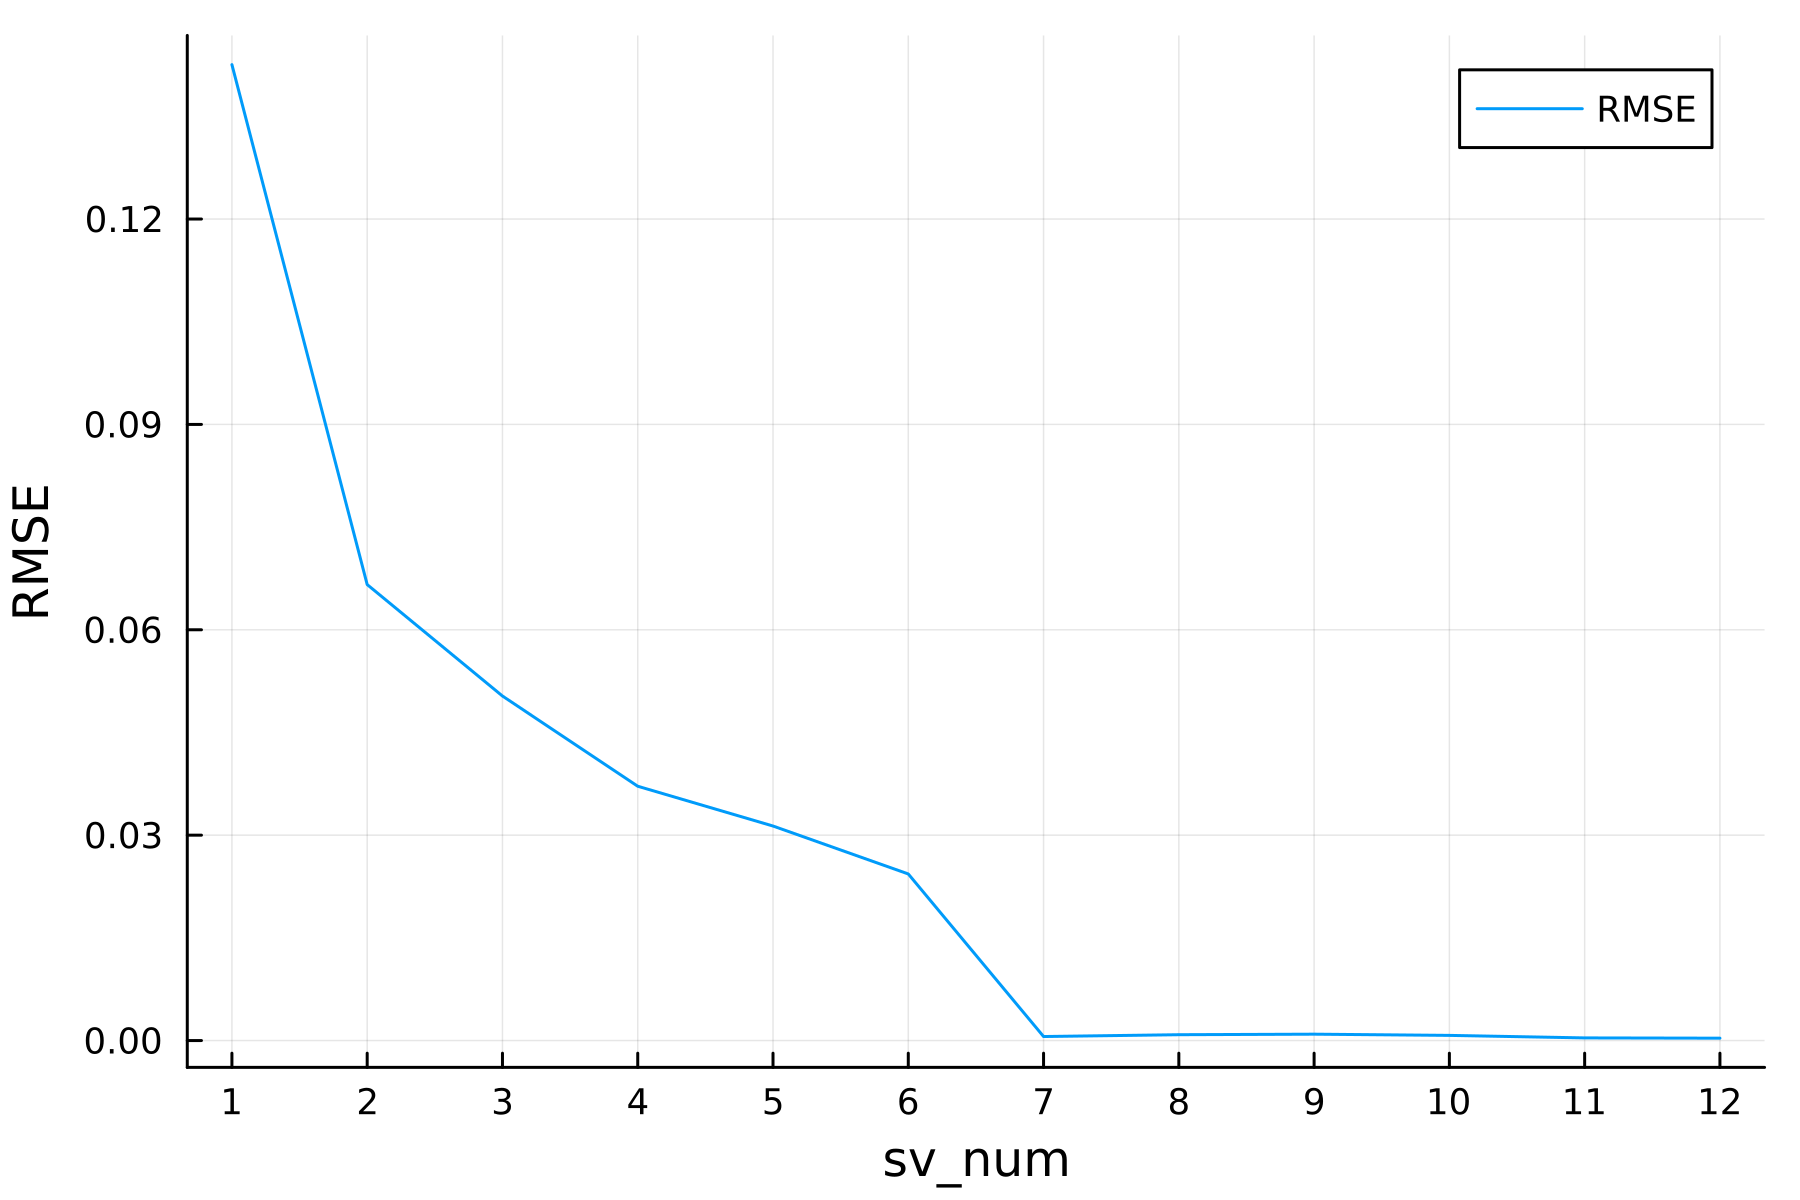
\includegraphics[width=\linewidth]{../RMSE.png}
			\caption{Без шумов}
		\end{subfigure}
		\begin{subfigure}{0.4\textwidth}
			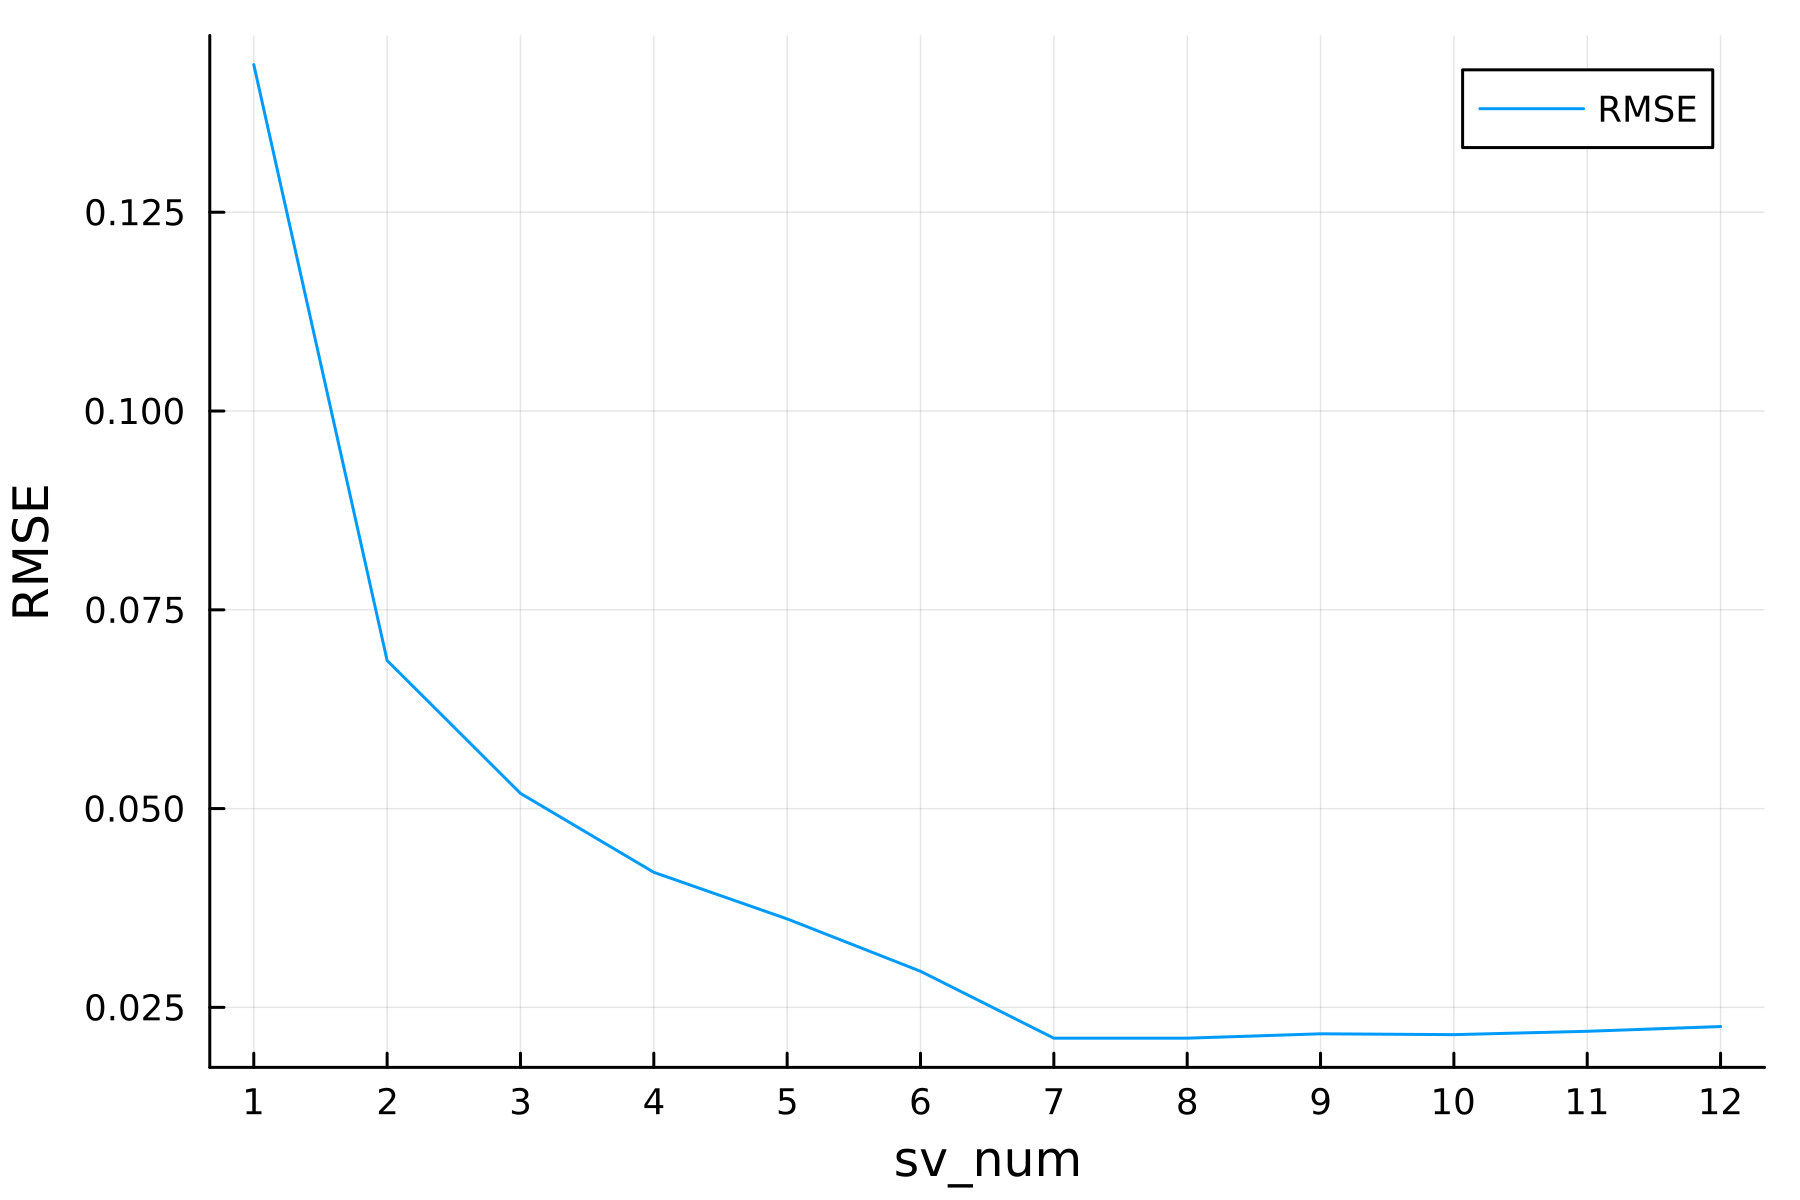
\includegraphics[width=\linewidth]{../RMSE_noise.png}
			\caption{С шумом}
		\end{subfigure}
		\caption{Графики зависимости ошибки от количества опорных векторов}
	\end{figure}
\end{frame}

\begin{frame}
	\frametitle{Выводы}
	\begin{itemize}
		\item Из графиков видно, что 7 - оптимальное количество опорных векторов для
		      этих данных, так как без шума модель идентична $sinc(x)$, также по
		      графикам зависимости СКО от количества опорных векторов видно, что после 7
		      ошибка особо не уменьшается.
		\item На графике зависимости ошибки от количества опорных векторов на
		      данных с шумом, можно заметить, что после 10 ошибка немного начинает
		      возрастать. Это можно связать с тем, что минимизация целевой функции
		      происходит жадно, то есть, мы не всегда получаем истинный минимум.

		\item В общем и целом, алгоритм показал себя хорошо, взамен
		      на небольшую ошибку в точности из-за жадности, мы получаем большой прирост
		      в производительности.

	\end{itemize}

\end{frame}

\end{document}
